\chapter{Methodology}
\label{chap:methodology}

\noindent\textbf{Document purpose:} Minor-report draft for advisor progress review.\\
\textbf{Reporting cutoff:} 16 September 2026.\\
\textbf{Evidence basis:} Current repository source, configuration, launch files,
generated artifacts, and dated engineering records.\\
\textbf{Status:} Draft. Implementation claims have been checked against the
repository; literature citations and faculty-specific thesis formatting remain to
be completed.

\section{Progress Scope and Implemented System Overview}
\label{sec:method-overview}

This project investigates vision-based localization for an autonomous mobile
robot in a dynamic warehouse. At the reporting cutoff, the implemented work
compares two stereo-inertial front ends, ORB-SLAM3 and VINS-Fusion, using common
simulated or recorded sensor streams. A custom YOLO detector can be enabled to
prevent image features associated with selected warehouse-object classes from
entering pose estimation. RTAB-Map is used as a separate back end when persistent
map construction, loop closure, pose-graph correction, or localization against a
saved database is studied.

\begin{figure}[htbp]
  \centering
  \resizebox{\textwidth}{!}{% Experimental architecture. Nodes are placed on an explicit grid rather than by
% relative chaining: the detector sits between the two estimators so that its two
% optional edges are short verticals instead of connectors routed through the
% estimator boxes, and every arrow enters a distinct face of its target node.
% The trajectory-to-RTAB-Map gap is sized to hold its edge label clear of both
% boxes and of the grouping rectangle.
\begin{tikzpicture}[
  block/.style={draw, rounded corners, align=center, minimum height=9mm,
    text width=34mm, font=\footnotesize, fill=implemented, inner sep=2mm},
  source/.style={block, fill=gray!15},
  backend/.style={block, fill=external},
  plan/.style={block, fill=planned, dashed},
  flow/.style={-{Latex[length=2.2mm]}, thick},
  optional/.style={flow, dashed},
  edgelabel/.style={font=\scriptsize, fill=white, inner sep=1.5pt}
]
  \node[source]  at ( 0.0,  0.0) (sensors)    {Stereo images\\and IMU};
  \node[block]   at ( 5.0,  2.8) (vins)       {VINS-Fusion\\track culling and\\feature suppression};
  \node[block]   at ( 5.0,  0.0) (detector)   {Optional YOLO\\box detector};
  \node[block]   at ( 5.0, -2.8) (orb)        {ORB-SLAM3\\feature rejection};
  \node[source]  at (10.2,  0.0) (trajectory) {Common trajectory\\\texttt{vio.csv}};
  \node[backend] at (16.6,  0.0) (rtab)       {RTAB-Map\\external back end};
  \node[source]  at (10.2, -5.0) (evaluation) {Trajectory and\\map evaluation};
  \node[plan]    at (16.6, -5.0) (future)     {Planned integrated\\relocalization, global\\optimization, map merging};

  % Sensor stream reaches the detector and both estimators without crossings.
  \draw[flow] (sensors.east) -- (vins.west);
  \draw[flow] (sensors.east) -- (detector.west);
  \draw[flow] (sensors.east) -- (orb.west);

  % Optional masks: short verticals, so nothing is drawn across a box.
  \draw[optional] (detector.north) -- (vins.south);
  \draw[optional] (detector.south) -- (orb.north);

  % Both estimators write the common trajectory; they enter the two left corners
  % so the arrowheads stay apart and the south face is free for the next edge.
  \draw[flow] (vins.east) -- (trajectory.north west);
  \draw[flow] (orb.east) -- (trajectory.south west);
  \draw[flow] (trajectory.south) -- (evaluation.north);
  \draw[flow] (trajectory.east) -- node[edgelabel]{TF odometry} (rtab.west);
  \draw[flow] (rtab.south west) -- (evaluation.east);
  \draw[optional] (rtab.south) -- (future.north);

  \node[draw, fit=(vins)(orb)(trajectory), inner sep=3mm,
    label={[font=\scriptsize]above:front-end trajectory path}] {};
\end{tikzpicture}
}
  \caption{Implemented experimental architecture. Green blocks are implemented
  project components, blue denotes the external RTAB-Map back end, and the dashed
  yellow block is future work. The diagram deliberately does not show a feedback
  connection from RTAB-Map into either front end because that integration has not
  been implemented.}
  \label{fig:system-architecture}
\end{figure}

As shown in \cref{fig:system-architecture}, the current work contains two related
but separate evaluation paths. The first measures front-end trajectory behaviour
with and without semantic feature filtering. The second studies map reconstruction
and external global correction through RTAB-Map. RTAB-Map's
\texttt{map~$\rightarrow$~odom} transform does not modify the internal feature map,
state history, or previously recorded trajectory of ORB-SLAM3 or VINS-Fusion. A
unified architecture for relocalization, global optimization, and multi-session
map merging is \status{planned}, not implemented. Path planning is outside the
present research scope.

\begin{longtable}{>{\raggedright\arraybackslash}p{0.30\textwidth}
                  >{\raggedright\arraybackslash}p{0.23\textwidth}
                  >{\raggedright\arraybackslash}p{0.39\textwidth}}
\caption{Implementation status at the reporting cutoff.}
\label{tab:implementation-status}\\
\toprule
Component & Status & Scope of evidence \\
\midrule
\endfirsthead
\toprule
Component & Status & Scope of evidence \\
\midrule
\endhead
Warehouse simulation and controlled worlds & \status{Implemented; verified} &
Static, dynamic, textured-floor, and featureless-floor world and launch files are
present. \\
ORB-SLAM3 ROS~2 stereo-inertial wrapper & \status{Implemented; verified in
simulation} & Live topics, worker-thread tracking, TF, and common trajectory
output are implemented. \\
ORB-SLAM3 semantic filtering & \status{Implemented; mechanism verified} &
Detector messages reach the tracker and masked ORB candidates are rejected before
octree distribution. \\
VINS-Fusion stereo-inertial estimator & \status{Implemented} & Simulation and
real-rig configurations, odometry publication, TF, and trajectory output are
present. \\
VINS-Fusion semantic filtering & \status{Implemented; mechanism verified} &
Existing KLT tracks are culled and new features are suppressed in detected
regions. \\
Offline YOLO evaluation & \status{Implemented; partially evaluated} &
Ground-truth projection, IoU matching, per-frame CSV files, and validation
overlays are present. \\
RTAB-Map construction and saved-map localization & \status{Implemented; partially
verified} & Construction and basic read-only localization passed; one tiny-map
database has been quantitatively evaluated for geometry and drivability
(\cref{sec:map-quality}). Arbitrary-start aliasing rejection and the
large-warehouse evaluation have not been done. \\
RTAB-Map extend and multi-session merging & \status{Implemented at launch level;
experimentally unverified} & The mode exists, but the planned Level~4 experiment
has not been completed. \\
Live VINS-Fusion and RTAB-Map co-execution & \status{Blocked} & VINS diverges under
the combined workload on the current computer; the mechanism is unresolved. \\
RPE and complete compute evaluation & \status{Partially implemented} & Front-end,
back-end, local-mapping, loop-closing, delivery/state, cumulative process CPU,
and resident-memory records are now logged. RPE was added after the cutoff and
applied to the campaign (\cref{sec:rpe}). External-process monitoring and the
repeated hardware matrix remain planned. \\
\bottomrule
\end{longtable}

The repository state used for this draft is superproject commit
\repo{4425a415f624d6a45da1da4f3b2404cbf7914197}. The checked-out submodules are
VINS-Fusion \repo{4a2223c9e54dfc5d2e94eb2ec1dfc8fd3b8045bb}, RTAB-Map ROS
\repo{56064e4388f6f3ad6b994dbff98bcc0a41488102}, and the warehouse environment
\repo{3df54c6e6ec267fad204e208db61c4ab491be410}. The ORB-SLAM3 core is pinned to
\repo{5c2b00f732775f78836751dba13db25463a0aaa1}. The VINS-Fusion worktree contains
an uncommitted output-directory creation fix at the cutoff; this must be committed
or otherwise recorded before a reproducibility release.

\section{Hardware, Software, Sensors, Calibration, and Frames}
\label{sec:platform-calibration}

\subsection{Computing and software environment}

Development and recorded experiments use Ubuntu 22.04.5, ROS~2 Humble, GCC
11.4.0, CMake 3.22.1, and system OpenCV 4.5.4. The recorded development machine
has 16 logical CPU cores, 15~GB RAM, no swap, and an NVIDIA RTX~3070 Laptop GPU.
The detector environment recorded in the engineering log contains PyTorch
2.5.1+cu121, torchvision 0.20.1, Ultralytics 8.4.138, NumPy 1.26.4, and Python
OpenCV 4.11. ORB-SLAM3 is built out of tree with Pangolin 0.9.1. RTAB-Map uses the
apt core library \repo{ros-humble-rtabmap} 0.23.7 with the project checkout of its
ROS wrappers; only wrapper packages through \repo{rtabmap_slam} are built.

These specifications describe the current laptop, not a completed cross-hardware
experiment. The proposed Jetson-versus-laptop study has not been instrumented or
executed, so no hardware comparison is inferred from the present data.

\subsection{Simulated sensor rig}

The simulated Ackermann robot carries two ideal pinhole cameras and an IMU on a
forward mast, and is driven through a front-steering, rear-driven four-wheel
chassis. \Cref{fig:ackermann-robot} gives its dimensioned plan and elevation, and
\cref{tab:sim-sensor-rig,tab:platform-geometry} list the sensor and platform
constants. Every value in the figure and both tables is read from
\repo{aws-robomaker-small-warehouse-world/models/ackermann_robot/model.sdf}, so
the drawing is to scale rather than illustrative.

\begin{figure}[htbp]
  \centering
  \resizebox{\textwidth}{!}{% Dimensioned plan and elevation of the simulated Ackermann robot.
%
% Every coordinate below is read from
% aws-robomaker-small-warehouse-world/models/ackermann_robot/model.sdf and is
% expressed in metres relative to base_footprint, so the drawing is to scale and
% can be re-derived from the model rather than trusted. A Gazebo screenshot was
% deliberately not used: the quantities that matter to the estimators are the
% wheel base, track, wheel radius and sensor offsets, and a perspective render
% shows none of them.
%
% NOTE ON THE TWO VIEWS. They are placed side by side with shift={(1.45,0)},
% i.e. in DIAGRAM units, not with yshift/xshift in centimetres. Inside a scope
% that already carries scale=9 a shift given in cm is multiplied by that scale,
% which silently pushes the second view about 56 cm away and off the page.
\begin{tikzpicture}[
  scale=9,
  chassis/.style={draw, fill=gray!12, thick},
  wheel/.style={draw, fill=gray!45, thick},
  steered/.style={draw, dashed, gray!60!black, line width=0.4pt},
  mast/.style={draw, fill=gray!25},
  sensor/.style={draw, fill=external, thick},
  imu/.style={draw, fill=implemented, thick},
  dim/.style={{Latex[length=1.2mm]}-{Latex[length=1.2mm]}, gray!60!black,
    line width=0.3pt},
  dimlab/.style={font=\tiny, inner sep=1pt, fill=white},
  leader/.style={gray!60!black, line width=0.25pt},
  lbl/.style={font=\tiny, inner sep=1pt},
  tick/.style={gray!60!black, line width=0.25pt}
]

% ======================= PLAN VIEW (x forward, y left) =======================
\begin{scope}
  \node[font=\small\bfseries] at (0.15,0.44) {Plan view};

  % chassis deck: 0.6 x 0.463 centred on base_footprint
  \draw[chassis] (-0.3,-0.2315) rectangle (0.3,0.2315);

  % steered front wheels shown at full lock, +/-0.6109 rad = +/-35 deg,
  % rotated about the kingpin rather than drawn as a bare angle sweep
  \foreach \y in {0.21,-0.21}{
    \begin{scope}[shift={(0.21,\y)}, rotate=35]
      \draw[steered] (-0.0585,-0.0325) rectangle (0.0585,0.0325);
    \end{scope}
  }

  % wheels: radius 0.0585, half-width 0.0325, at x = +/-0.21, y = +/-0.21
  \foreach \x in {0.21,-0.21}{
    \foreach \y in {0.21,-0.21}{
      \draw[wheel] (\x-0.0585,\y-0.0325) rectangle (\x+0.0585,\y+0.0325);
    }
  }
  \node[lbl, anchor=south west] at (0.135,0.275)
    {$\delta_{\max}=\pm\SI{0.6109}{\radian}$};

  % camera mast and the two cameras
  \draw[mast] (0.3078,-0.01) rectangle (0.5395,0.01);
  \draw[sensor] (0.486,0.0836) rectangle (0.506,0.1036);
  \draw[sensor] (0.486,-0.01) rectangle (0.506,0.01);

  % IMU
  \draw[imu] (0.313,-0.025) rectangle (0.363,0.025);
  \node[lbl, anchor=north] at (0.338,-0.032) {\texttt{imu}};

  % base_footprint origin marker
  \draw[thick] (-0.025,0) -- (0.025,0) (0,-0.025) -- (0,0.025);
  \node[lbl, anchor=north] at (0,-0.035) {\texttt{base\_footprint}};

  % camera labels, lifted clear on leaders so they cannot collide with the
  % baseline dimension between them
  \draw[leader] (0.506,0.0936) -- (0.60,0.155);
  \node[lbl, anchor=west] at (0.605,0.155) {\texttt{cam0} (left)};
  \draw[leader] (0.506,0) -- (0.60,-0.075);
  \node[lbl, anchor=west] at (0.605,-0.075) {\texttt{cam1} (right)};

  % --- dimensions ---
  \draw[tick] (0.21,-0.2425) -- (0.21,-0.315);
  \draw[tick] (-0.21,-0.2425) -- (-0.21,-0.315);
  \draw[dim] (-0.21,-0.30) -- (0.21,-0.30);
  \node[dimlab] at (0,-0.30) {wheel base \SI{0.42}{\metre}};

  \draw[tick] (-0.2685,0.21) -- (-0.375,0.21);
  \draw[tick] (-0.2685,-0.21) -- (-0.375,-0.21);
  \draw[dim] (-0.36,-0.21) -- (-0.36,0.21);
  \node[dimlab, rotate=90] at (-0.36,0) {track \SI{0.42}{\metre}};

  \draw[tick] (0.506,0.0936) -- (0.565,0.0936);
  \draw[tick] (0.506,0) -- (0.565,0);
  \draw[dim] (0.552,0) -- (0.552,0.0936);
  \node[dimlab, rotate=90] at (0.552,0.047) {\SI{0.0936}{\metre}};
\end{scope}

% ======================= ELEVATION (x forward, z up) =======================
\begin{scope}[shift={(1.45,-0.16)}]
  \node[font=\small\bfseries] at (0.15,0.60) {Side elevation};

  % ground line
  \draw[gray!55, line width=0.5pt] (-0.38,0) -- (0.60,0);

  % wheels seen edge on: centre z = 0.072, radius 0.0585
  \foreach \x in {0.21,-0.21}{
    \draw[wheel] (\x,0.072) circle (0.0585);
    \draw[gray!60!black, line width=0.25pt] (\x,0.072) circle (0.007);
  }

  % chassis deck: z from 0.072 to 0.122
  \draw[chassis] (-0.3,0.072) rectangle (0.3,0.122);

  % mast: vertical post, camera bar, short riser
  \draw[mast] (0.399,0.122) rectangle (0.419,0.3715);
  \draw[mast] (0.3078,0.3715) rectangle (0.5395,0.3915);
  \draw[mast] (0.486,0.3915) rectangle (0.506,0.4295);

  % cameras at z = 0.4395 (cam0 hides cam1 in this projection)
  \draw[sensor] (0.482,0.4295) rectangle (0.510,0.4495);
  \draw[leader] (0.510,0.4395) -- (0.55,0.50);
  \node[lbl, anchor=west] at (0.555,0.50) {\texttt{cam0}, \texttt{cam1}};

  % IMU at z = 0.192
  \draw[imu] (0.313,0.182) rectangle (0.363,0.202);
  \draw[leader] (0.363,0.192) -- (0.44,0.25);
  \node[lbl, anchor=west] at (0.445,0.25) {\texttt{imu}, $z=\SI{0.192}{\metre}$};

  % --- dimensions ---
  \draw[dim] (0.21,0.072) -- (0.21,0.1305);
  \node[dimlab, anchor=west] at (0.222,0.101) {$r=\SI{0.0585}{\metre}$};

  \draw[tick] (0.510,0.4395) -- (0.585,0.4395);
  \draw[dim] (0.572,0) -- (0.572,0.4395);
  \node[dimlab, rotate=90] at (0.572,0.22) {\SI{0.4395}{\metre}};

  \draw[tick] (-0.2685,0.072) -- (-0.375,0.072);
  \draw[dim] (-0.36,0) -- (-0.36,0.072);
  \node[dimlab, rotate=90] at (-0.36,0.036) {axle \SI{0.072}{\metre}};
\end{scope}

\end{tikzpicture}
}
  \caption{Simulated Ackermann platform, drawn to scale from the model
  definition. Distances are in metres relative to \texttt{base\_footprint}. The
  stereo pair is mounted asymmetrically: \texttt{cam1} sits on the vehicle
  centreline and \texttt{cam0} is offset \SI{0.0936}{\metre} to its left, so the
  optical centre of the pair is not the chassis centreline. The wheel base and
  track are equal at \SI{0.42}{\metre}, which is what makes the rear-wheel
  differential a poor yaw-rate estimator (\cref{sec:proprio-method}).}
  \label{fig:ackermann-robot}
\end{figure}

\begin{table}[htbp]
\centering
\caption{Simulated sensor configuration. Intrinsics are analytic rather than
calibrated: the simulator renders an exact pinhole camera, so $f_x=f_y$ follow
from the image width and the horizontal field of view and the distortion
coefficients are identically zero. The stereo baseline was independently checked
from positive disparity in a recorded bag rather than taken from the model alone.}
\label{tab:sim-sensor-rig}
\small
\resizebox{\textwidth}{!}{%
\begin{tabular}{llll}
\toprule
Quantity & \texttt{cam0} (left) & \texttt{cam1} (right) & \texttt{imu} \\
\midrule
Resolution & $1280\times720$ & $1280\times720$ & -- \\
Rate & \SI{30}{\hertz} & \SI{30}{\hertz} & \SI{200}{\hertz} \\
Horizontal FOV & $\pi/2$ rad (\SI{90}{\degree}) & $\pi/2$ rad (\SI{90}{\degree}) & -- \\
$f_x=f_y$ & 640 & 640 & -- \\
$(c_x,c_y)$ & $(640,360)$ & $(640,360)$ & -- \\
Distortion & zero & zero & -- \\
Position from \texttt{base\_footprint} (m) & $(0.496,0.0936,0.4395)$ &
  $(0.496,0,0.4395)$ & $(0.338,0,0.192)$ \\
Position from IMU body (m) & $(0.158,0.0936,0.2475)$ & $(0.158,0,0.2475)$ &
  $(0,0,0)$ \\
Stereo baseline & \multicolumn{2}{l}{\SI{0.0936}{\metre}} & -- \\
\bottomrule
\end{tabular}}
\end{table}

The fixed camera rotation converts the ROS body convention (forward, left, up) to
the optical convention (right, down, forward). The VINS simulation configuration
fixes the extrinsics (\repo{estimate_extrinsic: 0}) and disables temporal-offset
estimation (\repo{estimate_td: 0}); the assumed inertial noise model is given in
\cref{tab:imu-noise-assumed}, and the same values are mapped to the ORB-SLAM3
configuration.

\begin{table}[htbp]
\centering
\caption{Inertial noise parameters supplied to the visual-inertial estimators,
beside the values measured from the recorded IMU stream in
\cref{sec:proprio-method}. The configured values are inherited estimator defaults,
not measurements of this simulated IMU; the discrepancy is carried forward as a
queried item rather than silently reconciled.}
\label{tab:imu-noise-assumed}
\small
\begin{tabular}{llll}
\toprule
Parameter & Configured (VINS, ORB) & Measured from bag & Units \\
\midrule
\texttt{acc\_n} & 0.02 & \flag{0.0139--0.0294} &
  m\,s$^{-2}/\sqrt{\mathrm{Hz}}$ \\
\texttt{gyr\_n} & 0.002 & \flag{0.000300--0.000364} &
  rad\,s$^{-1}/\sqrt{\mathrm{Hz}}$ \\
\texttt{acc\_w} & 0.001 & not measurable & m\,s$^{-3}/\sqrt{\mathrm{Hz}}$ \\
\texttt{gyr\_w} & 0.0001 & not measurable &
  rad\,s$^{-2}/\sqrt{\mathrm{Hz}}$ \\
\bottomrule
\end{tabular}
\end{table}

\begin{queried}[Queried]
The configured gyroscope noise density is \num{2e-3} whereas the stationary
windows of the five recorded streams give \numrange{3.00e-4}{3.64e-4}, so the
configured value is about six times too large. The configured accelerometer
density of 0.02 sits inside the measured spread but that spread is itself wide,
\numrange{0.0139}{0.0294} across five bags of the same simulated sensor. Both
estimators are therefore running on an inertial noise model that does not
describe this IMU closely. The bias random walks cannot be checked at all: the
longest stationary interval in any \repo{dataset_allsensor} bag is
\SI{1.54}{\second} and an Allan-variance estimate needs minutes. No conclusion in
this report depends on these four numbers, but they should be re-derived from a
dedicated stationary recording before any tuning claim is made.
\end{queried}

\begin{queried}[Queried]
The accelerometer characterisation is not stable across recordings of the same
simulated sensor. \repo{allsensor_002}, whose stationary window is
\SI{1.54}{\second} and therefore the best conditioned of the three, returns an $x$
bias of \SI{0.0683}{\metre\per\second\squared}, against 0.0191 for
\repo{allsensor_000} and \SI{0.0016}{\metre\per\second\squared} for
\repo{allsensor_004}, whose window is the shortest at \SI{0.52}{\second}. The
scale ranges from 1.0199 to 1.0669 over the five. Because the window is short in
every case, part of this spread is estimator variance rather than a property of
the sensor, and the accelerometer terms should not be quoted as calibrated
constants. The gyroscope scale agrees to four decimal places across all five bags;
its bias does not, varying by a factor of twenty, which is consistent with the
same window-length problem.
\end{queried}

\begin{table}[htbp]
\centering
\caption{Platform geometry and drivetrain limits used by the wheel-odometry and
EKF baselines. \texttt{AckermannSteering} exposes no noise parameter, so the
simulated encoders and odometry are noise free at source.}
\label{tab:platform-geometry}
\small
\begin{tabular}{llll}
\toprule
Quantity & Symbol & Value & Source field \\
\midrule
Wheel base (front to rear axle) & $L$ & \SI{0.42}{\metre} & \texttt{wheel\_base} \\
Track (wheel separation) & $B$ & \SI{0.42}{\metre} & \texttt{wheel\_separation} \\
Kingpin width & -- & \SI{0.42}{\metre} & \texttt{kingpin\_width} \\
Wheel radius & $r$ & \SI{0.0585}{\metre} & \texttt{wheel\_radius} \\
Wheel width & -- & \SI{0.065}{\metre} & wheel \texttt{<length>} \\
Steering limit & $\delta_{\max}$ & $\pm\SI{0.6109}{\radian}$ & \texttt{steering\_limit} \\
Chassis mass & -- & \SI{10.1}{\kilogram} & \texttt{base\_footprint} \texttt{<mass>} \\
Maximum speed & -- & \SI{10}{\metre\per\second} & \texttt{max\_velocity} \\
Maximum acceleration & -- & \SI{3}{\metre\per\second\squared} & \texttt{max\_acceleration} \\
Odometry publish rate & -- & \SI{50}{\hertz} & \texttt{odom\_publish\_frequency} \\
Joint-state publish rate & -- & \SI{1}{\kilo\hertz} & measured from bag \\
\bottomrule
\end{tabular}
\end{table}

\subsection{Simulation fidelity and its limits}
\label{sec:sim-fidelity}

Every simulation result in this report rests on how faithfully the simulator
reproduces the sensors and the contact physics. This subsection states what is
modelled, what is idealised, and in which direction each idealisation biases the
comparison between the visual and proprioceptive estimators.

\paragraph{Inertial measurement.} \Cref{tab:imu-noise-assumed} reports the noise
measured from the recorded stream and queries it, because no
\repo{dataset_allsensor} bag contains a stationary interval long enough for a
sound estimate. That query can be closed without a new recording: the noise is
\emph{declared}, not emergent, so the simulator's own configuration is the
ground truth the measurement was trying to recover.

The \repo{<imu>} sensor block injects zero-mean Gaussian noise at
\SI{200}{\hertz} with per-sample standard deviations of
\SI{0.0048}{\radian\per\second} and
\SI{0.0566}{\metre\per\second\squared} --- densities of \num{3.394e-4} and
\num{4.002e-3} in their respective units per $\sqrt{\si{\hertz}}$. The measured
gyroscope range of \numrange{3.00e-4}{3.64e-4} brackets the declared value, which
corroborates both. The measured accelerometer range of
\numrange{1.39e-2}{2.94e-2} does not: it is three to seven times the declared
figure, and the discrepancy is the estimator's, not the sensor's, since the
residual on the driving axis carries real longitudinal acceleration that a
1.54\,\si{\second} window cannot separate from noise. The declared values should
be preferred wherever a number is needed.

Against the ADIS16448 of the EuRoC benchmark, on which both estimators were
published, the simulated unit is \emph{twice as noisy} on both channels, so it is
not an optimistic sensor. Bias is first-order Gauss--Markov with correlation
times of \SI{1000}{\second} and \SI{300}{\second}.

The IMU is therefore not optimistic in its noise. Three things are nonetheless
absent: chassis vibration, which on a real platform is frequently the dominant
error; scale-factor, cross-axis and $g$-sensitivity errors; and temperature
drift. The correlation times also exceed the \SIrange{85}{130}{\second} run
lengths, so within a run the bias behaves as a slowly varying constant and its
instability is never exercised. Finally, the message's \repo{orientation} field
carries no noise block at all and is therefore ground truth; no estimator in this
project consumes it, and none should.

\paragraph{Wheel encoders.} \repo{JointStatePublisher} reports the true solver
angle. Slip consequently appears as a \emph{discrepancy} rather than an error ---
the joint angle stays true, so encoder-integrated distance over-reads whenever
traction breaks, which is exactly a real encoder's behaviour. What is idealised
is resolution: a physical 1024\,CPR encoder quantises to \SI{6.1e-3}{\radian},
setting a floor on low-speed velocity estimation that the simulation does not
have. \repo{script/encoder_sim.py} exists to impose that floor downstream and has
not been applied to any result in this report.

\paragraph{Contact friction, and why the encoder is flattered.} ODE uses the
smaller friction coefficient of the two contacting surfaces. The wheels declare
$\mu=1$, $\mu_2=1$; every ground model declares $\mu=100$, $\mu_2=50$; so the
contact runs at $\mu=1.0$, the optimistic end of the published dry-clean-concrete
range. Force-dependent slip is disabled, \repo{slip1} and \repo{slip2} being
pinned at zero on all three ground models, so contact is rigid until Coulomb
traction is exceeded.

\Cref{tab:measured-slip} gives the consequence, measured rather than assumed, by
integrating rear-wheel angle against true path length.

\begin{table}[htbp]
\centering
\caption{Measured wheel slip on the five multi-sensor recordings. The ratio is
encoder-integrated distance over true path length; above one is slip, below one
is a rolling-radius error and cannot be slip. Measured by
\repo{script/check_slip.py}.}
\label{tab:measured-slip}
\small
\begin{tabular}{lrrr}
\toprule
Recording & Encoder (m) & Truth (m) & Ratio \\
\midrule
\repo{allsensor_000} & 117.12 & 117.05 & 1.0006 \\
\repo{allsensor_001} & 112.91 & 113.11 & 0.9982 \\
\repo{allsensor_002} & 115.37 & 115.20 & 1.0015 \\
\repo{allsensor_003} & 141.68 & 140.61 & 1.0076 \\
\repo{allsensor_004} & 142.36 & 142.25 & 1.0008 \\
\bottomrule
\end{tabular}
\end{table}

Slip is present but under \SI{1}{\percent} everywhere, and on
\repo{allsensor_001} the encoder under-reads, which cannot be slip. Against a
wheel-odometry drift of \SIrange{2.15}{6.57}{\percent}, slip is therefore not the
dominant error; the yaw-rate geometry is, as the falsification of H1 establishes.

\begin{queried}[Threat to validity]
This is a bias with a known direction. The EKF baseline of
\cref{sec:results-proprio} is evaluated on a floor where the wheels effectively
cannot slip and with an encoder of unlimited resolution, which is dead
reckoning's best case. Both idealisations favour the EKF over the visual
estimators, and neither has been relaxed. The conclusion that a wheel+IMU filter
outperforms both visual pipelines should be read as holding \emph{under these
conditions}, not as a general result. \repo{script/make_slippery_floor.py}
generates ground models at a chosen friction coefficient so that traction can be
made an experimental factor; \repo{script/encoder_sim.py} imposes a realistic
quantisation floor. Neither has been used in any result reported here.
\end{queried}

\paragraph{Noise models supplied to the estimators.} The two are not told the
truth about the IMU. Both configurations set
\repo{acc_n}~$=\SI{0.02}{}$ and \repo{gyr_n}~$=\SI{0.002}{}$, over-stating the
injected densities by \num{5.0} and \num{5.9} times respectively, and
\repo{gyr_w} by a factor of \num{58}. Inflating noise above datasheet values is
standard practice in visual-inertial odometry, and the configuration records that
intent. The EKF baseline, by contrast, derives its noise model by measuring it
against ground truth from the same recording.

That asymmetry was tested directly rather than left as a caveat. Configurations
carrying the true injected densities --- \repo{stereo_imu_truenoise.yaml} for
both estimators --- were run on all five recordings on 18 September 2026, after
the reporting cutoff. Accuracy improved wherever a run completed: VINS-Fusion on
four of five, by \SI{43}{\percent} and \SI{32}{\percent} on two of them. But
three of ten runs diverged outright, reaching \SIrange{111}{3899}{\metre} of
error with \numrange{516}{1545} tracking jumps, where the inflated configuration
diverged in none. The behaviour is bimodal rather than graded: surviving runs
carry zero to three jumps, failed runs hundreds. This confirms the configuration
comment's own claim that too-large noise degrades gracefully while too-small does
not, and the inflated setting is retained for every result in this report. These
runs are recorded as \repo{logging_20260916_03} and are not part of the reported
campaign.

\subsection{Real sensor rig and calibration limits}

The real configuration is summarised in \cref{tab:real-rig}. Its calibration is
materially weaker than the simulated rig's, and the weaknesses are load bearing
rather than cosmetic.

\begin{table}[htbp]
\centering
\caption{Real sensor rig, and the calibration status of each quantity. Only the
first three rows are measured; the remainder are approximations or placeholders
that bound what can be claimed from real-robot data.}
\label{tab:real-rig}
\small
\begin{tabularx}{\textwidth}{>{\raggedright\arraybackslash}p{0.26\textwidth}>{\raggedright\arraybackslash}p{0.30\textwidth}>{\raggedright\arraybackslash}X}
\toprule
Quantity & Value & Status \\
\midrule
Stereo resolution & $1920\times1080$ fisheye & measured \\
Stereo baseline & \SI{0.093604}{\metre} & measured \\
IMU stream & \repo{/hwt101ct_yaw_publisher} & separate RealSense source \\
Camera model (ORB-SLAM3) & \texttt{KannalaBrandt8} & configured \\
Camera model (VINS) & project fisheye files & configured \\
Second-camera intrinsics & reuse of the first camera & \flag{approximation} \\
IMU-to-camera rotation & observational support & partial \\
IMU-to-camera translation & zero & \flag{placeholder} \\
Stationary $\lVert a\rVert$ & \SI{9.2642}{\metre\per\second\squared} &
  \flag{measured, deviates from \num{9.81}} \\
Extrinsic estimation (VINS) & \repo{estimate_extrinsic: 1} & online \\
Time-offset estimation (VINS) & \repo{estimate_td: 1} & online \\
\bottomrule
\end{tabularx}
\end{table}

The real IMU-to-camera rotation has observational support, but its translation is
a zero placeholder. The stationary accelerometer magnitude is recorded as
\SI{9.2642}{\metre\per\second\squared}, rather than
\SI{9.81}{\metre\per\second\squared}. VINS-Fusion uses the observed magnitude as
\repo{g_norm}; the ORB-SLAM3 real inertial launch rescales acceleration by
$9.81/9.2642$. These treatments make the configurations internally consistent but
do not replace an independent camera--IMU calibration. Real trajectories can be
inspected for plausibility and tracking continuity, but metric accuracy cannot be
claimed without independent ground truth and improved extrinsic calibration.

\subsection{Coordinate-frame contract}

Standalone VINS-Fusion publishes \texttt{world~$\rightarrow$~body}. Standalone
ORB-SLAM3 publishes an estimator-specific world frame. For RTAB-Map integration,
both publish \texttt{odom~$\rightarrow$~vio\_body}; a measured static transform
connects \texttt{vio\_body~$\rightarrow$~base\_footprint} by
$(-0.338,0,-0.192)$~m. RTAB-Map then publishes the external correction
\texttt{map~$\rightarrow$~odom} (\cref{fig:frame-chain}).

\begin{figure}[htbp]
  \centering
  \resizebox{\textwidth}{!}{% Coordinate-frame chain. Edge labels are lifted clear of the node row and the
% calibration-check edge is routed beneath the chain, so that no label or
% connector is drawn on top of a frame box.
\begin{tikzpicture}[
  node distance=8mm,
  frame/.style={draw, rounded corners, fill=implemented, minimum height=8mm,
    minimum width=24mm, align=center},
  sensor/.style={frame, fill=gray!15},
  flow/.style={-{Latex[length=2.2mm]}, thick},
  edgelabel/.style={font=\scriptsize, inner sep=1pt}
]
  \node[frame, fill=external] (map) {\texttt{map}};
  \node[frame, right=of map] (odom) {\texttt{odom}};
  \node[frame, right=of odom] (body) {\texttt{vio\_body}};
  \node[frame, right=of body] (foot) {\texttt{base\_footprint}};
  \node[frame, right=of foot] (base) {\texttt{base\_link}};
  \node[sensor, below=16mm of base] (cam0) {\texttt{cam0\_optical}};
  \node[sensor, right=of cam0] (cam1) {\texttt{cam1\_optical}};

  % The labelled gaps are only 8 mm wide, so each label is raised 6 mm above the
  % arrow: it then sits entirely above the 8 mm-tall boxes instead of over them.
  \draw[flow] (map) -- node[edgelabel, above=6mm]{RTAB-Map correction} (odom);
  \draw[flow] (odom) -- (body);
  \draw[flow] (body) -- node[edgelabel, above=6mm]{measured offset} (foot);
  \draw[flow] (foot) -- (base);
  \draw[flow] (base) -- (cam0);
  \draw[flow] (base) -- (cam1);

  % Consistency check, routed below the chain so it does not cross
  % base_footprint or base_link.
  \draw[flow, dashed] (body.south) |-
    node[edgelabel, above, pos=0.72]{runtime identity check} (cam0.west);
\end{tikzpicture}
}
  \caption{Coordinate-frame contract used by the composed RTAB-Map pipeline. The
  dashed connection is a calibration consistency check, not a second pose
  publisher.}
  \label{fig:frame-chain}
\end{figure}

The two independent paths to \texttt{cam0\_optical} provide a runtime calibration
check: \repo{tf2_echo cam0_undis cam0_optical} must return zero translation and
the identity quaternion. This check has been measured successfully. It is needed
because an earlier OpenCV YAML parsing error yielded a plausible translation but
a non-rigid rotation and invalidated a map-quality campaign.

The standalone simulation ORB launch still labels the estimated IMU-body pose as
\texttt{base\_footprint}. The composing RTAB-Map launch corrects this by using
\texttt{vio\_body}; standalone consumers must not assume that the default label is
the chassis origin. Constant offsets are mostly absorbed by rigid trajectory
alignment but remain material for map placement and robot-footprint tests.

\section{Environments, Datasets, and Controlled Factors}
\label{sec:environments-datasets}

\subsection{Simulation environment}

The principal large warehouse is a \SI{41.2833}{\metre} square environment
produced by rescaling the AWS warehouse to \SI{1704}{\metre\squared}, while
retaining a \SI{9.020}{\metre} interior height. Fourteen marked storage bays and
five reduced-width walkways are represented. Static and dynamic families are
stored under \repo{worlds/small_warehouse_static/} and
\repo{worlds/small_warehouse_dynamic/}. The original tiny warehouse under
\repo{worlds/small_warehouse/} is a distinct environment; tiny- and large-layout
results are not repeated trials of the same condition.

The occupancy truth of the object arrangements is shown in
\cref{fig:warehouse-maps}. These grids are not SLAM products: they are rasterised
directly from the world's collision meshes by \repo{script/bake_map.py}, sliced at
robot height, so they contain no unknown space and regenerate whenever the world
changes. They are the reference against which any reconstructed map is scored.

\begin{figure}[htbp]
  \centering
  \begin{minipage}[t]{0.32\textwidth}
    \centering
    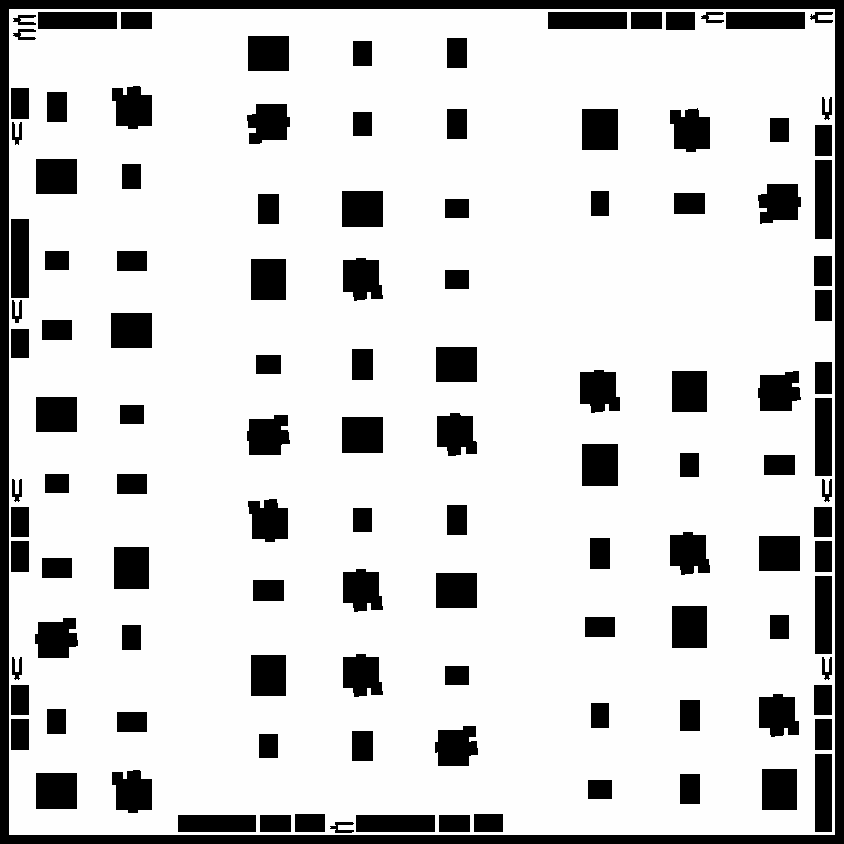
\includegraphics[width=\textwidth]{figures/warehouse_static_01.png}\\[0.4ex]
    {\footnotesize (a) static \texttt{\_01}, distributed}
  \end{minipage}\hfill
  \begin{minipage}[t]{0.32\textwidth}
    \centering
    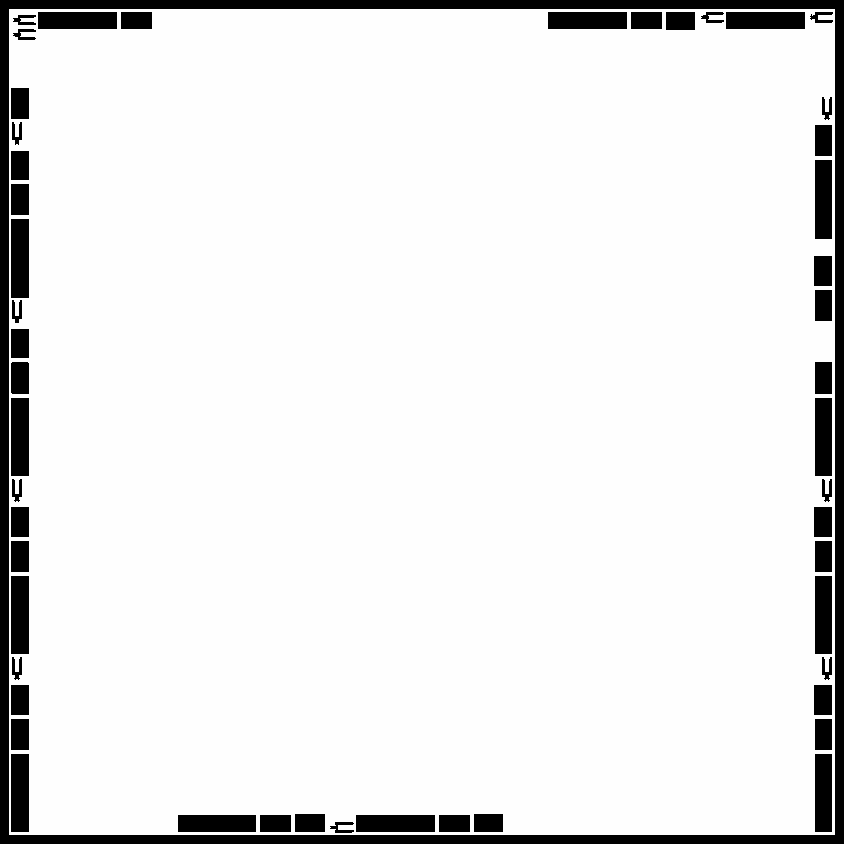
\includegraphics[width=\textwidth]{figures/warehouse_objonwallonly.png}\\[0.4ex]
    {\footnotesize (b) \texttt{objonwallonly}}
  \end{minipage}\hfill
  \begin{minipage}[t]{0.32\textwidth}
    \centering
    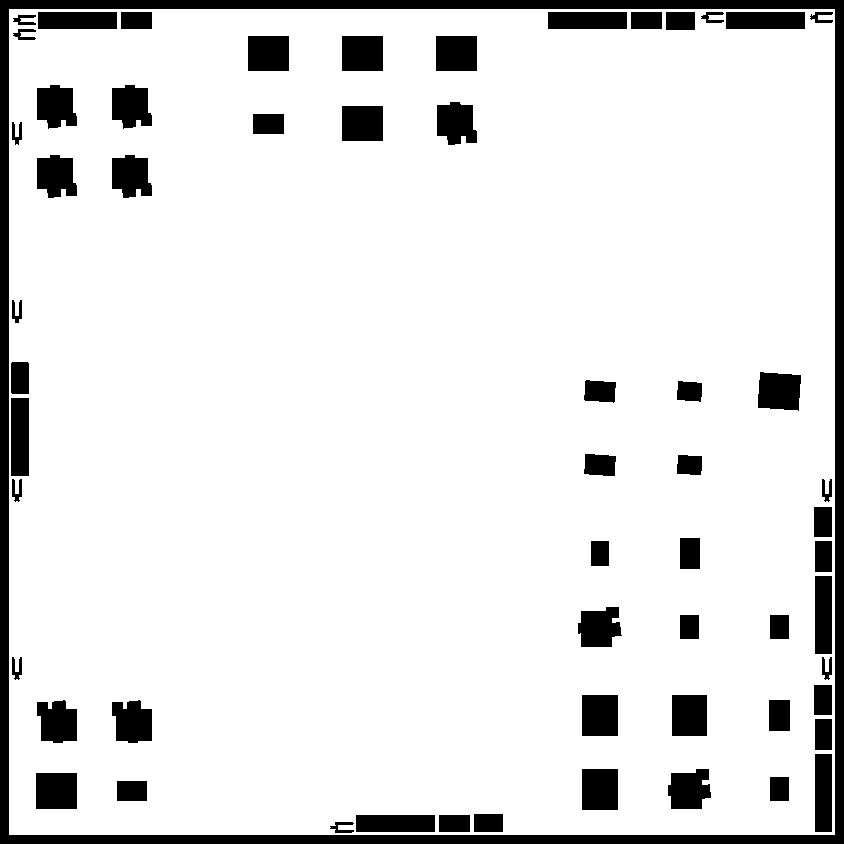
\includegraphics[width=\textwidth]{figures/warehouse_dynamic.png}\\[0.4ex]
    {\footnotesize (c) dynamic}
  \end{minipage}
  \caption{Baked occupancy truth of the three large-warehouse object arrangements,
  each \SI{42.2}{\metre} square at \SI{0.05}{\metre} per cell with origin
  $(-21.1,-21.1)$~m. Black is occupied, white is free; there is no unknown space
  because the grids are rasterised from collision geometry rather than observed.
  Occupied cells are \SI{17.79}{\percent} of~(a), \SI{8.74}{\percent} of~(b) and
  \SI{10.98}{\percent} of~(c). Panel~(b) clears the central floor and keeps
  obstacles against the walls, which is the arrangement used by
  \repo{dataset_allsensor_002} and \repo{dataset_allsensor_003}. \emph{No
  occupancy grid is shown per floor treatment, and none exists:} the
  \texttt{bayline} and plain floors differ only in surface material, which carries
  no collision geometry, so their baked grids are identical to the panels above.
  See \cref{fig:floor-treatments}.}
  \label{fig:warehouse-maps}
\end{figure}

The floor treatment is a separate factor and is invisible to occupancy. It is set
by which ground model a world includes; those models share one mesh and differ only
in the visual materials attached to it (\cref{tab:floor-variants}).
\Cref{fig:floor-treatments} renders both recorded conditions at true scale using
\repo{script/render_floor.py}, which drives the 2-D viewer's own floor rasteriser
so that the figure shows what the overlay and the simulated cameras see rather
than a texture file out of context.

\begin{figure}[htbp]
  \centering
  \begin{minipage}[t]{0.33\textwidth}
    \centering
    
\includegraphics[width=\textwidth]{figures/floor_plain.png}\\[0.4ex]
    {\footnotesize (a) plain, \repo{allsensor_000}--\repo{_002}}
  \end{minipage}\hfill
  \begin{minipage}[t]{0.33\textwidth}
    \centering
    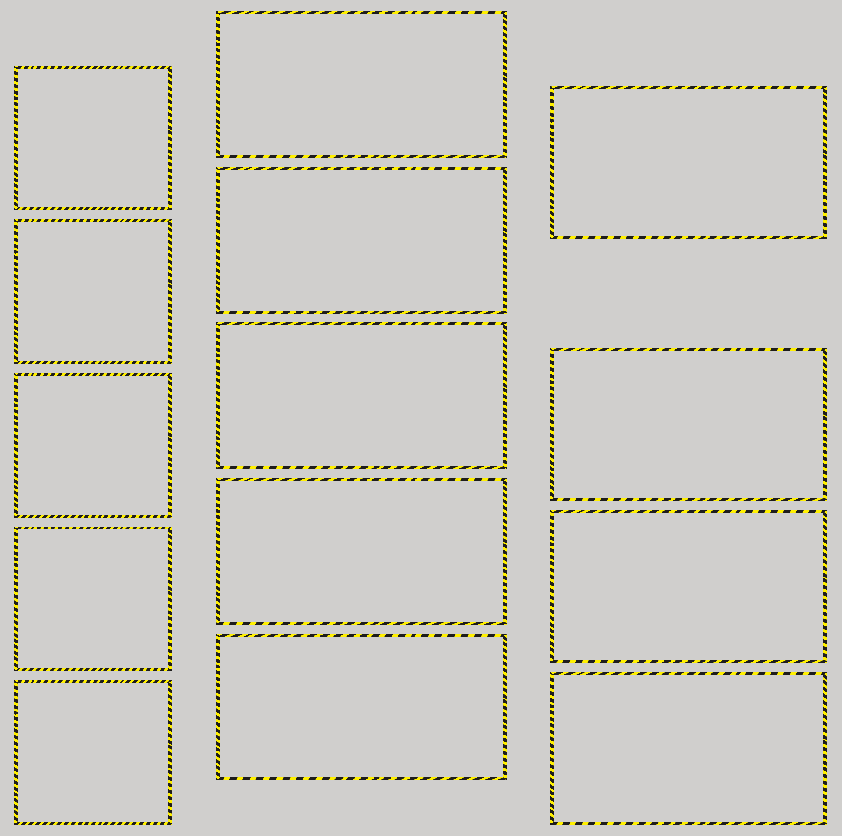
\includegraphics[width=\textwidth]{figures/floor_bayline.png}\\[0.4ex]
    {\footnotesize (b) \texttt{bayline}, \repo{allsensor_003}, \repo{_004}}
  \end{minipage}\hfill
  \begin{minipage}[t]{0.29\textwidth}
    \centering
    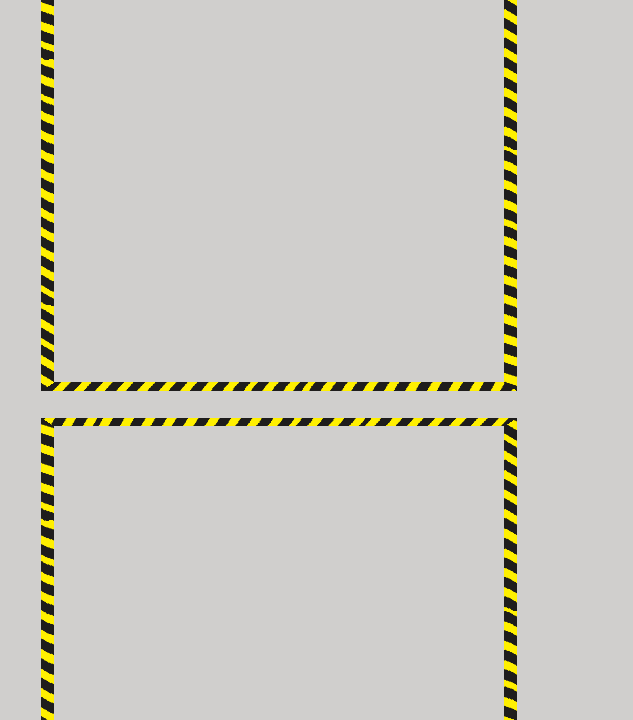
\includegraphics[width=\textwidth]{figures/floor_bayline_detail.png}\\[0.4ex]
    {\footnotesize (c) \SI{12}{\metre} detail of~(b)}
  \end{minipage}
  \caption{The two recorded floor conditions, rendered across the full
  \SI{42.2}{\metre} floor at \SI{0.05}{\metre} per pixel. Both share the same flat
  diffuse base, RGB $(0.814,0.811,0.804)$; the only difference between them is the
  112 painted marking faces that \texttt{bayline} adds, forming the hazard-striped
  outlines of fourteen storage bays. Panel~(c) is a \SI{12}{\metre} square detail
  showing the strips at \SI{0.145}{\metre} width. Everything not outlined is
  untextured in both conditions.}
  \label{fig:floor-treatments}
\end{figure}

\begin{table}[htbp]
\centering
\caption{Ground models and the floor conditions they produce. The mesh and its
collision geometry are identical in all three, so the floor treatment changes what
a camera sees and nothing a wheel, an occupancy grid or a collision check responds
to. The concrete-grain texture belongs to the stock model only, and no recorded
dataset uses it.}
\label{tab:floor-variants}
\small
\begin{tabularx}{\textwidth}{>{\raggedright\arraybackslash}p{0.29\textwidth}lll>{\raggedright\arraybackslash}X}
\toprule
Ground model & Base & Concrete & Markings & Used by \\
\midrule
\repo{..._GroundB_01} (stock) & texture & yes & 112 faces & no recorded dataset \\
\repo{..._GroundB_01_bayline} & flat diffuse & no & 112 faces &
  \repo{allsensor_003}, \repo{allsensor_004} \\
\repo{..._GroundB_01_plain} & flat diffuse & no & none &
  \repo{allsensor_000}--\repo{_002}, all \texttt{nofloortexture} datasets \\
\bottomrule
\end{tabularx}
\end{table}

\begin{queried}[Naming]
The factor recorded in this project as ``textured versus featureless floor'' is
narrower than the name suggests, and \cref{fig:floor-treatments} is the evidence.
Both conditions rest on the \emph{same flat, untextured diffuse colour}; the stock
concrete-grain texture appears in neither. The entire difference is fourteen
painted bay outlines, \SI{0.145}{\metre} wide, covering a small fraction of a
\SI{1704}{\metre\squared} floor. A robot driving an aisle sees a uniform grey
surface in both conditions for most of its path, crossing a high-contrast strip
only at a bay boundary.

Results comparing the two floors must therefore be read as \emph{bay markings
versus nothing}, not as \emph{realistic floor versus nothing}, and the near-absence
of a visual-odometry improvement between them (\cref{sec:results-proprio}) should
not be generalised to floors carrying genuine surface texture. Testing that would
require a world built on the stock \repo{GroundB_01} model, which no recorded
dataset uses.
\end{queried}

\begin{queried}[Unverified]
The dynamic world's baked grid, \cref{fig:warehouse-maps}(c), contains
\SI{38}{\percent} fewer occupied cells than the distributed static arrangement
in~(a). \repo{bake_map.py} rasterises every \texttt{<include>} in the
world file at its authored pose, so kinematically driven props should appear at
their initial positions, but this has not been confirmed for the dynamic family.
Until it is, panel~(c) must not be used as occupancy truth for scoring a
reconstructed map of a dynamic scene: the deficit may be a genuine difference in
static stocking, or it may be props missing from the bake, and those two
possibilities imply opposite corrections. The estimator results in
\cref{sec:results-proprio} are unaffected, as they use the arrangements in
panels~(a) and~(b) only.
\end{queried}

The available controlled factors are summarised in \cref{tab:controlled-factors}.

\begin{table}[htbp]
\centering
\caption{Controlled experimental factors available in the simulation environment,
with the levels realised at the reporting cutoff. A factor is listed as exercised
only where a recorded dataset exists for more than one of its levels.}
\label{tab:controlled-factors}
\small
\begin{tabularx}{\textwidth}{>{\raggedright\arraybackslash}p{0.21\textwidth}>{\raggedright\arraybackslash}p{0.30\textwidth}>{\raggedright\arraybackslash}X}
\toprule
Factor & Levels & Status at cutoff \\
\midrule
Scene dynamics & static props; scripted dynamic props & exercised \\
Floor markings & bay outlines present (\texttt{bayline});
  absent (plain) & exercised; no dataset carries surface texture \\
Prop or route arrangement & canonical; \texttt{\_00}; \texttt{\_01};
  \texttt{\_02} & exercised \\
Stocking level & partial; fully stocked static & fully stocked recorded \\
Object placement & distributed; restricted to the wall region & exercised, three
  bags to one \\
Domain & simulation; real robot & exercised, no real ground truth \\
World scale & tiny \repo{small_warehouse}; large rescaled families & distinct
  environments, never pooled \\
\bottomrule
\end{tabularx}
\end{table}

The plain floor removes the painted bay outlines; neither recorded condition
carries the stock concrete texture. Collision geometry and occupancy truth are
preserved in both (\cref{tab:floor-variants}). Dynamic props follow
deterministic routes through a kinematic Gazebo plugin. This preserves repeatable
motion and acceptable real-time factor, but it does not reproduce physical
collision response if the robot overlaps a moving prop.

World identity is recorded by exact \texttt{.world} path. ROS launches require
\repo{colcon build --symlink-install}; a plain build can leave an obsolete copied
world in \repo{install/}. When object motion is required by the 2-D viewer, model
poses must also be bridged from the simulator.

\subsection{Dataset registry}

Datasets are held in two places and the registry must cover both: the workspace
tree \repo{dataset/} and a removable drive mounted at
\repo{/media/ambushee/32E4AAB1E4AA772F/}, whose simulation bags sit under
\repo{dataset/} and whose real-robot recordings sit at its root.
\Cref{tab:dataset-registry} lists all eighteen recordings across both locations.
Six exist in one place only on the drive, seven in the workspace only, and three
are held in both.

\begin{sidewaystable}[p]
\centering
\caption{Complete dataset registry at the reporting cutoff, across both storage
locations. The \texttt{bayline} families carry a textured floor; every other
simulation entry is featureless. ``WS'' is the workspace tree \repo{dataset/} and ``FD'' the removable
drive; a size is given where that location holds a copy. ``Prop.'' marks the
proprioceptive group (\repo{/model/ackermann_robot_001/joint_state} and
\repo{/model/ackermann_robot_001/odometry}); ``IMU'' counts inertial messages,
on \repo{/imu} for simulation and \repo{/hwt101ct_yaw_publisher} for the real
rig. Durations are rosbag wall-clock recording durations: the simulator ran below
real time, so a bag's sim-time span is shorter than the figure shown. Integrity
was checked by opening each SQLite store and counting rows against the count its
\repo{metadata.yaml} declares, not by trusting the metadata.}
\label{tab:dataset-registry}
\scriptsize
\setlength{\tabcolsep}{4pt}
\begin{tabular}{llrrrrcccl}
\toprule
Dataset & Family & WS & FD & Dur.\ (s) & Messages & \texttt{/clock} & Truth &
  Prop. & Integrity \\
 & & (MB) & (MB) & & & & & & \\
\midrule
\repo{dataset_allsensor_000} & static \texttt{\_01} & 689 & -- & 129.3 & 211\,811 &
  \checkmark & \checkmark & \checkmark & ok \\
\repo{dataset_allsensor_001} & static \texttt{\_01} & 674 & -- & 126.2 & 198\,873 &
  \checkmark & \checkmark & \checkmark & ok \\
\repo{dataset_allsensor_002} & static, wall only & 750 & -- & 105.5 & 215\,528 &
  \checkmark & \checkmark & \checkmark & ok \\
\repo{dataset_allsensor_003} & bayline, wall only & 1056 & -- & 141.2 & 255\,699 &
  \checkmark & \checkmark & \checkmark & ok \\
\repo{dataset_allsensor_004} & bayline, distributed & 1311 & -- & 168.6 & 253\,942 &
  \checkmark & \checkmark & \checkmark & ok \\
\midrule
\repo{dataset_static_nofloortexture_000} & static & -- & 592 & 101.5 & 118\,597 &
  \checkmark & \checkmark & -- & ok \\
\repo{dataset_static_nofloortexture_001} & static & 617 & 1 & 92.0 & 113\,332 &
  \checkmark & \checkmark & -- & \flag{FD stub, WS ok} \\
\repo{dataset_static_nofloortexture_002} & static & -- & 688 & 103.3 & 122\,386 &
  \checkmark & \checkmark & -- & ok \\
\repo{dataset_static_nofloortexture_objonwallonly} & static, wall only & 648 & -- &
  110.5 & 114\,523 & \checkmark & \checkmark & -- & ok \\
\midrule
\repo{dataset_dynamic_nofloortexture_00_000} & dynamic \texttt{\_00} & -- & 653 &
  100.3 & 111\,988 & \checkmark & \checkmark & -- & ok \\
\repo{dataset_dynamic_nofloortexture_00_001} & dynamic \texttt{\_00} & -- & 778 &
  167.7 & 114\,169 & \checkmark & \checkmark & -- & ok \\
\repo{dataset_dynamic_nofloortexture_01_000} & dynamic \texttt{\_01} & 713 & 710 &
  165.4 & 126\,790 & \checkmark & \checkmark & -- & \flag{FD malformed, WS ok} \\
\repo{dataset_dynamic_nofloortexture_02_000} & dynamic \texttt{\_02} & -- & 758 &
  172.1 & 134\,995 & \checkmark & \checkmark & -- & ok \\
\midrule
\repo{dataset_map_01} & mapping, large & 818 & -- & 193.5 & 152\,291 & \checkmark &
  \checkmark & -- & ok \\
\repo{dataset_map_tiny} & mapping, tiny world & 726 & -- & 63.3 & 82\,555 &
  \checkmark & \checkmark & -- & ok \\
\midrule
\repo{dataset_real_000} & real rig & 2964 & 2964 & 116.6 & 36\,166 & -- & -- & -- &
  ok, 23\,257 IMU \\
\repo{dataset_real_001} & real rig & -- & 2099 & 85.5 & 9\,629 & -- & -- & -- &
  \flag{0 IMU messages} \\
\repo{dataset_real_002} & real rig & -- & 2869 & 113.5 & 12\,682 & -- & -- & -- &
  \flag{0 IMU messages} \\
\bottomrule
\end{tabular}
\end{sidewaystable}

The seven featureless-floor simulation bags of the relogged campaign
(\cref{sec:results-validity}) are the static and dynamic families listed above;
five were read from the drive and two from the workspace, for the reason recorded
next.

\begin{queried}[Data integrity]
Two drive copies are unreadable while presenting a complete, plausible
\repo{metadata.yaml}. \repo{dataset_static_nofloortexture_001} is a
\SI{524288}{\byte} stub whose metadata nevertheless declares 113\,332 messages,
and \repo{dataset_dynamic_nofloortexture_01_000} is \SI{710}{\mega\byte}---within
\SI{0.4}{\percent} of its workspace counterpart---with a valid SQLite header but a
store that reports \emph{database disk image is malformed} on any query. Both have
intact workspace copies, which is why those two datasets were read from the
workspace in the relogged campaign.

The general lesson is recorded as a control rather than an incident:
\repo{metadata.yaml} is written when recording begins and does not describe what
survived, so message counts, durations and topic lists copied from it are not
evidence that a bag is intact. Storage health must be established by opening the
SQLite store and counting rows, which is now part of the pre-experiment inspection
in \cref{sec:collection-validity}.
\end{queried}

\begin{queried}[Scope limit]
Only the five \repo{dataset_allsensor} bags carry wheel encoders and wheel
odometry; the other thirteen recordings omit those topics entirely. The
proprioceptive baseline of \cref{sec:results-proprio} therefore cannot be computed
for any dynamic condition, for the mapping bags, or for the real rig, and the
comparison between proprioception and visual odometry exists only in
\emph{static, featureless-floor} scenes---the conditions least favourable to
vision and most favourable to dead reckoning. Extending it requires re-recording
with the two topics bridged, not new analysis.
\end{queried}

\begin{queried}[Excluded]
\repo{dataset_real_001} and \repo{dataset_real_002} are excluded because their
inertial topic \repo{/hwt101ct_yaw_publisher} contains \emph{zero} messages, so
neither supports stereo-inertial operation at all. Their image streams are intact
(2\,562 and 3\,405 pairs), so they remain usable for detector or image-only work.
\repo{dataset_real_000} is the only real recording with inertial data, at 23\,257
messages.
\end{queried}

Historical output folders do not prove that their raw bags remain available or
valid. Conversely, a dataset is not marked broken merely because its only copy
lives on the removable drive rather than in the repository; six of the fifteen
recordings are drive-only and are sound.

Before a new experiment, the bag's absolute path, topics, duration, message
counts, and storage health are inspected. Each paired comparison uses the same
recording, and estimators run separately to avoid resource-contention effects.
Environment, trajectory, calibration, replay rate, image transport,
initialization treatment, and revision are controlled. A run is excluded if
input overlap, initialization, processed sample count, or sensor delivery differs
materially from its paired condition.

Recorded simulation bags used by RTAB-Map contain \texttt{/clock}. They are
played without rosbag's additional \texttt{--clock} option because competing
clock sources cause TF time jumps. This choice is made after inspecting each bag,
not applied as a universal command rule.

\section{ORB-SLAM3 and Semantic Feature Filtering}
\label{sec:orb-method}

The project provides a purpose-built ROS~2 Humble wrapper around the pinned
ORB-SLAM3 core. Approximate-time synchronization pairs left and right images with
a \SI{0.02}{\second} slop. Raw and compressed transports are supported. Image
callbacks place stereo pairs in a one-frame queue; a worker thread calls
\texttt{TrackStereo()} so blocking visual tracking does not starve the
\SI{200}{\hertz} IMU subscription. If tracking falls behind, the older pending
image is discarded and the drop count is reported.

With \repo{filter:=false}, no detection subscription is created and an empty mask
passes through the patched interfaces. With filtering enabled, a bounded buffer
is searched for the detection closest in source-image time, accepted only within
\SI{0.15}{\second}. Boxes are expanded by eight pixels, clipped to the image, and
rasterized to an 8-bit mask in which 255 retains a feature and zero rejects it. A
mask covering more than 0.8 of the frame is discarded as a safety measure.

The mask passes through \texttt{System}, \texttt{Tracking}, and \texttt{Frame} to
the ORB extractor. Candidate keypoints are tested before octree distribution, so
the per-level feature quota can be redistributed across surviving static regions.
At each pyramid level, the implemented boundary rule rejects a candidate when at
least five samples in a $3\times3$ neighbourhood are dynamic. Only left-camera
features are masked because ORB-SLAM3 establishes stereo matches from left
keypoints to right candidates.

The current simulation YAML requests 1,000 ORB features, eight pyramid levels, a
1.2 scale factor, initial FAST threshold 20, and fallback threshold 7. An older
engineering note states 1,500 features, but the current configuration is
authoritative. No controlled feature-count or FAST-threshold sweep is complete.

The wrapper publishes \repo{/orbslam3/odometry}, \repo{/orbslam3/pose}, and TF
after valid tracking. It writes the common 11-column trajectory format directly
and flushes each row. Repository evidence is located in
\repo{orbslam3_ros2/src/orbslam3_node.cpp},
\repo{orbslam3_ros2/src/slam_wrapper.cpp},
\repo{orbslam3_ros2/src/trajectory_writer.cpp}, and
\repo{orbslam3_ros2/config/wil_sim/stereo_imu.yaml}.

\section{VINS-Fusion and the RTAB-Map Back End}
\label{sec:vins-rtab-method}

\subsection{VINS-Fusion front end}

VINS-Fusion uses stereo features and inertial measurements in a sliding-window
nonlinear estimator. The ROS wrapper synchronizes the raw image topics and uses
separate callback groups for images, IMU, feature messages, and detections. The
simulation configuration processes every image (\repo{image_skip: 1}), uses two
cameras and IMU, fixes simulated extrinsics, targets \SI{25}{\hertz} feature
publication, and uses 10-pixel keyframe parallax. Image queues were increased to
100 and the IMU queue to 2,000 to reduce losses during initialization and backlog.

VINS cannot use only the ORB strategy because it propagates existing features
with pyramidal KLT optical flow and detects new features only for replenishment.
A feature attached to an object before detection could otherwise persist after
masking. The implementation initializes \texttt{FeatureTracker::setMask()} from
the YOLO mask. Tracks in zero-valued regions fail the retention test, while the
same mask is passed to \texttt{goodFeaturesToTrack()} to suppress new points. The
count of persistent tracks removed in dynamic regions is accumulated as a
mechanism diagnostic.

VINS writes the optimized state after each estimator update to \repo{vio.csv} and
broadcasts \texttt{world~$\rightarrow$~body} using configurable frame names. The
ROS \repo{output_path} parameter overrides the YAML path, recursively creates
missing directories, and reports an explicit error if \repo{vio.csv} cannot be
opened. This behaviour is an uncommitted worktree change at the cutoff. Evidence
is in \repo{vins_fusion_ros2/src/vins_estimator.cpp},
\repo{vins_fusion_ros2/vins/src/featureTracker/feature_tracker.cpp}, and
\repo{vins_fusion_ros2/vins/src/estimator/estimator.cpp}.

\subsection{RTAB-Map mapping and localization back end}

RTAB-Map receives front-end odometry through TF and stereo imagery through
\repo{rtab_camera_shim.py}. The shim reconstructs \texttt{CameraInfo}, decompresses
the pair, and publishes validated static camera transforms from the common
simulation calibration. TF was selected over an odometry topic because adding
high-rate odometry to multi-topic approximate synchronization starved the
lower-rate images. The cost is that odometry covariance is not supplied to graph
edge weighting.

The back end uses stereo SGBM (\repo{Stereo/DenseStrategy: 1}), height-based
ground separation, ray tracing, spatial noise filtering, and odometry-derived
gravity links. Its measured default depth range is \SI{10}{\metre}. Because the
featureless floor provides essentially no stereo ground points, ray tracing
supplies free-space evidence between the sensor and observed obstacles. These
settings affect occupancy assembly; visual-word loop closure is separate.

Three modes are provided by one launch file:
\begin{description}
  \item[construct] starts a new incremental database;
  \item[extend] opens an existing database, places prior nodes in working memory,
    and permits new nodes; and
  \item[localize] disables incremental memory, loads existing nodes, serves the
    saved map, and can enable \repo{Mem/LocalizationReadOnly}.
\end{description}

Localization still extracts features from current stereo images and matches
stored RTAB-Map signatures. Read-only mode prevents database modification; it
does not disable perception. The outputs are an external
\texttt{map~$\rightarrow$~odom} correction and \repo{/localization_pose}. Neither
RTAB-Map features nor corrected poses are injected into ORB-SLAM3's Atlas or
VINS-Fusion's sliding window.

The composed localization launch raises \repo{RGBD/OptimizeMaxError} from 3.0 to
10.0 because the default rejected all loop closures proposed with the observed
VINS drift. This is effective operationally but is not yet proven safe against
perceptual aliasing in repeated warehouse bays. Occupancy creation is disabled in
localization mode because the stored map is reused. Live VINS-Fusion and RTAB-Map
co-execution nevertheless remains blocked on the current machine. Recorded
\repo{vio.csv} can be replayed as \texttt{odom~$\rightarrow$~vio\_body} for a
deterministic back-end test, but this is not proof of real-time co-execution.

Evidence is in \repo{rtabmap_ros/rtab_sim.launch.py},
\repo{rtabmap_ros/rtab_camera_shim.py},
\repo{aws-robomaker-small-warehouse-world/launch/localization_rtabmap.launch.py},
and \repo{script/gt_tf_publisher.py}.

\section{Non-Visual Baseline Estimators}
\label{sec:proprio-method}

The visual estimators were, until the cutoff, scored only against ground truth.
That establishes how large their error is but not whether it is good, because no
alternative was measured on the same data. Three non-visual estimators were
therefore implemented in \repo{script/proprio_estimator.py} to supply a
dead-reckoning floor: wheel odometry, IMU dead reckoning, and an extended Kalman
filter fusing the two. They consume only proprioceptive topics and no images.

\subsection{Implementation form and why it is offline}

All three read the recorded bag directly and are deterministic functions of it.
Run as live ROS nodes they would instead depend on replay rate, QoS delivery and
CPU contention, none of which is a property of the estimator being compared. The
cost is a stated asymmetry: the visual figures they are compared against were
produced by live runs, so any timing-induced error is present on one side of the
comparison only. This is revisited in \cref{sec:results-proprio}.

\subsection{Sensor model derived from data}

Every covariance field in the source bags is identically zero---0 of 17\,416 IMU
messages, 0 of 4\,355 wheel-odometry messages, and 0 of 4\,354 ground-truth
messages in \repo{dataset_allsensor_000}. Gazebo Fortress does not populate them,
and \texttt{AckermannSteering} exposes no noise parameter. The noise model is
consequently measured rather than read, by a \repo{calibrate} step that writes
\repo{sensor_noise.yaml}; \cref{tab:proprio-noise} gives the result for both bags.

\begin{table}[htbp]
\centering
\caption{Sensor noise and scale measured from each bag by
\repo{proprio_estimator.py calibrate}. Scales are least-squares gains through the
origin against ground truth; $\sigma$ values are the residual standard deviations.
A scale of 1.0 is an unbiased sensor. The bias random walks are assumed, not
measured, because the longest stationary window is \SI{1.54}{\second}.}
\label{tab:proprio-noise}
\small
\resizebox{\textwidth}{!}{%
\begin{tabular}{llrrrrrl}
\toprule
Group & Quantity & \repo{\_000} & \repo{\_001} & \repo{\_002} & \repo{\_003} &
  \repo{\_004} & Units \\
 & & plain & plain & plain & bayline & bayline & \\
\midrule
IMU & gyroscope $z$ bias & $6.48\times10^{-5}$ & $7.75\times10^{-5}$ &
  $9.28\times10^{-5}$ & $6.09\times10^{-4}$ & $2.58\times10^{-5}$ & \si{\radian\per\second} \\
 & gyroscope $\sigma$ & $4.36\times10^{-3}$ & $4.24\times10^{-3}$ &
  $4.81\times10^{-3}$ & $5.03\times10^{-3}$ & $5.15\times10^{-3}$ & \si{\radian\per\second} \\
 & gyroscope $z$ scale & 0.9990 & 1.0000 & 1.0002 & 1.0002 & 1.0000 & -- \\
 & accelerometer $x$ bias & 0.0191 & 0.0304 & \flag{0.0683} & 0.0309 & 0.0016 &
  \si{\metre\per\second\squared} \\
 & accelerometer $x$ scale & 1.0199 & 1.0249 & \flag{1.0669} & \flag{1.0525} & \flag{1.0465} & -- \\
 & measured $g$ & 9.7809 & 9.8191 & 9.7827 & 9.8037 & 9.8346 & \si{\metre\per\second\squared} \\
\midrule
Wheel & speed scale & 1.0002 & 0.9985 & 1.0005 & 1.0071 & 1.0001 & -- \\
 & speed $\sigma$ & 0.0407 & 0.0484 & 0.0496 & 0.0607 & 0.0505 & \si{\metre\per\second} \\
 & yaw-rate scale, bicycle & 1.0110 & 0.9527 & 1.0034 & \flag{0.9375} & \flag{0.9250} & -- \\
 & yaw-rate $\sigma$, bicycle & 0.0659 & 0.0804 & 0.0705 & 0.1192 & 0.0613 &
  \si{\radian\per\second} \\
 & yaw-rate scale, differential & 1.2162 & 1.1442 & 1.2194 & 1.2748 & 1.1404 & -- \\
 & yaw-rate $\sigma$, differential & 0.2359 & 0.3074 & 0.2620 & 0.3477 & 0.2828 &
  \si{\radian\per\second} \\
\midrule
Window & static duration & 0.68 & 0.58 & 1.54 & 1.04 & \flag{0.52} & \si{\second} \\
 & maximum tilt & 0.0016 & 0.0018 & 0.0015 & 0.0018 & 0.0017 & \si{\degree} \\
\bottomrule
\end{tabular}}
\end{table}

Two consequences follow directly. First, wheel \emph{speed} is essentially
unbiased on all five bags (scale 1.0002 to 1.0071), so distance travelled is not
the error source. Second, the rear-wheel differential is a far worse yaw-rate estimator
than the steering-angle bicycle model---residuals of \SIrange{0.26}{0.35}{\radian\per\second}
against \numrange{0.061}{0.119}---because the track
and the wheel base are both \SI{0.42}{\metre} and a solid rear axle slips through
every turn. The bicycle model is selected automatically and was chosen on all five
bags.

\subsection{The orientation field must not be used}

\texttt{sensor\_msgs/Imu.orientation} in these bags is not an estimate. Measured
over \repo{dataset_allsensor_000} it equals ground-truth yaw minus exactly
\SI{90}{\degree}, with residual standard deviation \SI{0.00000}{\degree} and
\SI{0.00000}{\degree} of drift across \SI{87}{\second}: the plugin publishes the
true orientation from the simulator's entity-component manager. Consuming it
would give a ``dead-reckoning'' estimator a perfect attitude reference that no
real IMU has, and its output would measure ground truth. All three estimators
therefore integrate \texttt{angular\_velocity.z} instead, which drifts honestly by
\SI{2.52}{\degree} over \SI{87}{\second} on \repo{allsensor_000} and
\SI{1.70}{\degree} over \SI{81.8}{\second} on \repo{allsensor_001}. The same check
on \repo{allsensor_002} again returns a residual standard deviation of
\SI{0.000000}{\degree} against ground-truth yaw, so the exclusion is not specific
to the first two recordings. Each run
records \repo{imu_orientation_used=NO} in its metadata so the exclusion is
auditable.

\subsection{Estimator definitions}

\Cref{tab:proprio-estimators} defines the three estimators. The EKF carries the
planar state $\mathbf{x}=[p_x,p_y,\theta,v,b_\omega]^{\top}$, predicted at the
\SI{200}{\hertz} IMU rate and corrected at \SI{50}{\hertz} by the wheels.

\begin{table}[htbp]
\centering
\caption{Implemented non-visual estimators. ``Anchoring'' refers to the initial
pose: dead reckoning has no global reference, so all three start from the
ground-truth pose at their first sample, and this is recorded as an alignment
decision rather than treated as neutral.}
\label{tab:proprio-estimators}
\small
\begin{tabularx}{\textwidth}{>{\raggedright\arraybackslash}p{0.15\textwidth}>{\raggedright\arraybackslash}p{0.21\textwidth}>{\raggedright\arraybackslash}p{0.21\textwidth}>{\raggedright\arraybackslash}X}
\toprule
Estimator & Inputs & State & Correction \\
\midrule
Wheel odometry & rear wheel speeds, steering angles (\SI{1}{\kilo\hertz}) &
  $[p_x,p_y,\theta]$ & none; $\mathbf{P}$ grows without bound \\
IMU dead reckoning & gyroscope $z$, accelerometer $x$ (\SI{200}{\hertz}) &
  $[p_x,p_y,\theta,v]$ & none \\
EKF wheel + IMU & both of the above & $[p_x,p_y,\theta,v,b_\omega]$ & wheel speed
  corrects $v$; $(\omega_{\text{gyro}}-\omega_{\text{wheel}})$ corrects
  $b_\omega$ \\
\bottomrule
\end{tabularx}
\end{table}

The EKF's second measurement is deliberately an observation of the \emph{gyroscope
bias} and not of heading. Integrating the wheel yaw rate into a heading and
correcting $\theta$ with it would reproduce the wheel estimator inside the filter
and inherit its unbounded drift. Treating the instantaneous rate difference as an
observation of $b_\omega$ keeps each sensor supplying what it measures well: the
wheels know rate, the gyroscope knows change, and neither knows absolute heading,
so heading remains unobservable and its variance correctly continues to grow. The
update uses the Joseph form, which keeps $\mathbf{P}$ symmetric and positive
definite across the roughly 16\,000 updates in a run.

Measured scale errors are recorded but never divided out. Correcting them would
mean calibrating the estimator with the ground truth it is about to be scored
against; the scale error is a real property of encoder odometry and is retained.

\section{YOLO Model, Mask Construction, and Synchronization}
\label{sec:yolo-method}

The semantic front end is a standalone Python ROS~2 node using Ultralytics. The
project checkpoint is \repo{weight/best.pt}, a custom detector for \texttt{bin},
\texttt{box}, and \texttt{bucket}, fine-tuned from \repo{yolo26m.pt} using
640-pixel inputs. It produces bounding boxes, not segmentation masks. The stock
\repo{yolo26n.pt} and \repo{yolo26m.pt} files are not project-trained models and
are not evidence of custom training.

At startup, the node resolves requested classes against checkpoint metadata,
warms the model with three dummy images, and selects CUDA when available. Current
defaults are confidence 0.35, NMS IoU 0.5, and image size 640. Only the left image
is processed. Each \texttt{Detection2DArray} preserves the source image header,
so nearest-timestamp selection measures sensor-time correspondence rather than
inference-completion time. Empty arrays distinguish a valid frame with no
detections from detector failure.

The detector intentionally remains outside stereo synchronization. A three-input
image/image/detection synchronizer would discard pairs whenever inference lagged.
The implemented design continues without filtering if no recent detection exists.
Filtered runs write \repo{yolo_mask.csv} with timestamp, box count, coverage,
match state, detection age, and rejection status.

Offline evaluation in \repo{script/yolo_eval.py} transforms Gazebo model poses and
collision-mesh vertices into the left-camera frame to form projected truth boxes.
Object speed over \SI{0.05}{\metre\per\second} defines the moving subset.
Predictions are greedily matched by class at IoU 0.5. Heavily occluded truth boxes
and predictions covered by known but unlabeled box-like scenery are ignored at
stated thresholds. Outputs are per-frame \repo{yolo_eval.csv}, per-detection
\repo{yolo_detections.csv}, and overlays. Overlays are inspected before aggregate
metrics because invalid pose stamps, centimetre mesh units, or malformed camera
transforms can produce plausible but invalid numbers.

The current semantic rule assumes all selected-class detections are dynamic. No
optical-flow, stereo-depth, or world-motion gate is implemented, and axis-aligned
boxes also remove background pixels. These are explicit method limitations.

\section{Collection Protocol, Validity, and Artifacts}
\label{sec:collection-validity}

The sensor source, estimator, optional detector, and viewer start as separate
processes; launch files do not automatically play bags. Baseline and filtered
treatments run separately on the same recording, at a replay rate that permits
comparable input consumption. Competing estimators are not run simultaneously in
a scientific A/B comparison.

The common trajectory file has no header and uses:
\begin{center}
\texttt{t\_ns, px, py, pz, qw, qx, qy, qz, vx, vy, vz}
\end{center}
Timestamps are integer nanoseconds from the source header and quaternion order is
$w,x,y,z$. ORB-SLAM3 writes this representation directly; VINS writes the state
after nonlinear optimization. Simulation truth is extracted to the same shape by
\repo{script/extract_gt.py}. The tracker-use record \repo{yolo_mask.csv} remains
separate from the offline detector score.

\begin{table}[htbp]
\centering
\caption{Principal stored artifacts.}
\label{tab:stored-artifacts}
\small
\begin{tabularx}{\textwidth}{>{\raggedright\arraybackslash}p{0.42\textwidth}X}
\toprule
Artifact & Purpose \\
\midrule
\repo{<run>/vio.csv} & Estimator trajectory and velocity \\
\repo{<run>/ground_truth.csv} & Simulation reference trajectory, when available \\
\repo{<run>/yolo_mask.csv} & Actual mask matching, coverage, and rejection \\
\repo{<run>/run_metadata.csv} & Resolved configuration and supplied provenance \\
\repo{<run>/performance.csv} & Per-frame timing, state, delivery, CPU, and memory \\
\repo{<run>/frontend.csv} and \repo{<run>/backend.csv} & VINS feature-tracking,
estimator-stage, solver, and state-window diagnostics \\
\repo{<run>/tracking_frontend.csv} & ORB-SLAM3 tracking-stage timing and feature counts \\
\repo{<run>/local_mapping.csv} & ORB-SLAM3 keyframe insertion, map-point, and local-BA diagnostics \\
\repo{<run>/loop_closing.csv} & Place-recognition, loop, merge, and global-correction events \\
\repo{<run>/run_summary.csv} & Graceful-shutdown validity and robustness totals \\
\repo{<run>/events.csv} & VINS initialization, reset-cause, and shutdown events \\
\repo{output/yolo_eval/<experiment>/yolo_eval.csv} & Per-frame detector evaluation \\
\repo{output/yolo_eval/<experiment>/yolo_detections.csv} & Per-detection matching \\
\repo{output/yolo_eval/<experiment>/overlay/} & Projection and matching validation \\
\repo{map/*.db} or \repo{<run>/rtabmap.db} & Persistent RTAB-Map graph and signatures \\
\repo{output/compare/<domain>/<experiment>/} & Derived figures and summaries \\
\bottomrule
\end{tabularx}
\end{table}

The current analysis code requires at least ten overlapping samples. Scientific
acceptance additionally requires the same input interval, successful
initialization, comparable pose and frame counts, and no unexplained sensor
starvation. Steps implying over \SI{10}{\metre\per\second} are tracking jumps; an
indoor estimate with error beyond \SI{50}{\metre} is divergence rather than
ordinary inaccuracy. Without real-data ground truth, path length and mean speed
are plausibility diagnostics, not accuracy measurements.

The estimator now records resolved local configuration and optional experiment,
dataset, world, replay-rate, command, and note fields in
\repo{run_metadata.csv}. It does not automatically determine bag health,
repository revisions, complete dependency versions, external-process state, or
the analyst's exclusion decision. Empty optional fields therefore remain
incomplete provenance. Historical folders created before this instrumentation
remain preliminary unless their provenance is recoverable from logs and
engineering records.

\section{Evaluation Metrics and Analysis}
\label{sec:evaluation-method}

\subsection{Trajectory evaluation}
\label{sec:method-trajectory}

\repo{script/vio_metrics.py} associates estimate and reference over their common
time interval and interpolates the reference at estimator timestamps. A rigid
Umeyama $SE(3)$ fit maps estimated positions to the reference with scale fixed at
one. Fixed scale is appropriate for stereo-inertial estimators and preserves
scale error. Outputs include translational ATE RMSE, maximum and final error,
rotational geodesic error, path length, overlap duration, pose count, jump count,
and longest jump-free segment. Optional startup trimming is relative to each
estimator's first overlapping pose, preventing unequal initialization latency
from being interpreted as steady-state behaviour.

The older \repo{plot_vio_vs_gt.py} provides a first-pose-aligned diagnostic, but
headline comparison uses common $SE(3)$ alignment. Real data without independent
ground truth receives no ATE.

\paragraph{Relative pose error.} RPE was added to \repo{script/vio_metrics.py}
after the reporting cutoff, on 18 September 2026, and is
\status{implemented and exercised on the full campaign}. It follows the
conventional definition: for a pair of poses separated by a fixed interval
$\Delta$, the error transform is
\begin{equation}
  E_i = \left(Q_i^{-1}Q_{i+k}\right)^{-1}\left(P_i^{-1}P_{i+k}\right),
  \label{eq:rpe}
\end{equation}
with $P$ the estimate and $Q$ the reference. Translational RPE is
$\lVert\operatorname{trans}(E_i)\rVert$ and rotational RPE is the geodesic angle
of $\operatorname{rot}(E_i)$, the same angle measure used for orientation error
above.

RPE is reported because it needs \emph{no} global alignment, and that is what
makes it the appropriate metric for the dynamic runs. A single discontinuity
re-seats the rigid $SE(3)$ fit, so every subsequent pose inherits the offset and
ATE describes the jump rather than the tracking. RPE instead asks a local
question --- over the next $\Delta$ seconds, did the estimate move as the
reference moved --- and is insensitive to both the global frame and accumulated
drift. It therefore supersedes the longest-jump-free-segment statistic, which
answers a similar question through a segment-selection heuristic rather than a
standard definition.

Four intervals are swept, $\Delta \in \{0.5, 1, 2, 5\}\,\si{\second}$, giving
an error-versus-interval curve; $\Delta = \SI{1}{\second}$ is the headline value
and corresponds to roughly \SI{1.4}{\metre} at the simulated robot's cruising
speed. A pair is admitted only when its realised separation lies within
\SI{25}{\percent} of $\Delta$, so a gap in the log cannot silently widen the
interval and inflate the error; the surviving pair count is reported with every
statistic. Pairs are overlapping, which is the conventional default.

Each statistic is computed twice: over all admissible pairs, and over only those
pairs that do not span a detected tracking jump. The difference isolates the
teleport contribution from ordinary local error, mirroring the existing
separation between global and clean-segment ATE. Both RMSE and median are
reported, because the dynamic-run distributions are strongly right-skewed and a
single teleport otherwise sets the RMSE.

The implementation is verified against synthetic trajectories with known answers:
an estimate identical to the reference returns zero; a constant relative drift of
\SI{0.1}{\metre\per\second} returns \SI{0.100}{\metre} at
$\Delta=\SI{1}{\second}$ and \SI{0.200}{\metre} at $\Delta=\SI{2}{\second}$; a
\SI{2}{\degree\per\second} relative rotation returns \SI{2.00}{\degree} at
$\Delta=\SI{1}{\second}$; and an injected teleport separates the all-pairs and
jump-free statistics by the expected pair count. Results are written to
\repo{rpe_metrics.csv} for the interval sweep, with the
$\Delta=\SI{1}{\second}$ values carried into \repo{trajectory_metrics.csv}.

\subsection{Detection evaluation}

Detector precision, recall, TP, FP, FN, moving/static recall, IoU, and image-area
coverage are computed by \repo{yolo_eval.py} at recorded confidence, matching-IoU,
occlusion, minimum-size, and motion thresholds. Mask-use statistics are joined to
trajectories by \repo{timestamp_ns}. A semantic class is never treated as
ground-truth motion.

\subsection{Map and localization evaluation}

RTAB-Map grids are placed in the Gazebo world using one fixed rigid world-to-map
transform measured by \repo{script/fit_map_pose.py}. It is constant for a database;
the live \texttt{map~$\rightarrow$~odom} drift correction is not reused for map
placement.

\repo{script/validate_map.py} rasterizes world collision geometry and evaluates
occupied cells at a stated tolerance. It reports occupied-cell precision,
whole-world and observed-region recall, false obstacles under the true
$0.83\times0.50$~m footprint, unmapped footprint poses, and clearance. Graph
evaluation records neighbour, global-closure, local-space, and gravity links.
Localization additionally requires time to first fix, accepted and rejected
matches, database checksums before and after read-only operation, pose continuity,
and known-world bounds. Finite covariance or a localization status message alone
does not establish correctness.

At the cutoff this evaluation has been applied to one database,
\repo{map/map_tiny.db}, against
\repo{small_warehouse_static/small_warehouse_static_tinymap.world}. The
equivalent large-warehouse evaluation is \status{planned} and no database for
it exists; results are reported in \cref{sec:map-quality}.

\subsection{Computational performance}

Both estimator processes write per-frame \repo{performance.csv} files. These
record processing time, delivery and backlog counters, tracking or solver state,
initialization and reset evidence, pose and keyframe accounting, cumulative
process CPU time, monotonic wall time, and resident memory. VINS additionally
records feature-front-end and estimator-back-end stages; ORB-SLAM3 records its
tracking front end, local mapping, place recognition, loop closure, map merging,
and global bundle-adjustment events. CPU utilization and throughput can therefore
be derived over explicit wall-time intervals. The measurements are process-local
and exclude Gazebo, rosbag, RViz, RTAB-Map, and the separate YOLO process.
Synchronized whole-system monitoring and the repeated Jetson/laptop matrix
remain \status{planned}. Module timings from asynchronous stages are reported as
separate distributions and are not added as if they formed one serial critical
path.

\section{Reproducibility Controls and Implementation Deviations}
\label{sec:reproducibility-deviations}

The following controls govern future experiments and acceptance of historical
results:
\begin{enumerate}
  \item Record absolute bag and exact \texttt{.world} file, treatment,
    configuration, commands, clock and replay rate, hardware, dependencies, and
    relevant repository commits.
  \item Use a unique output directory and retain failed runs with failure labels.
  \item Run paired treatments independently on the same sensor data and compare
    only their common valid interval.
  \item Record inputs, outputs, initialization, dropped frames, resets, tracking
    loss, warnings, and exclusion reasons.
  \item Validate camera order, transport, timestamps, metric scale, and every
    rigid transform before analysis.
  \item Inspect representative detector and map overlays before aggregate scores.
  \item Repeat nondeterministic RTAB-Map processing and report valid-run count;
    do not interpret differences within run-to-run variation as algorithmic.
  \item Keep estimator, back end, filtering, environment dynamics, floor texture,
    domain, and hardware separate unless their interaction is the declared factor.
  \item Record every switch that changes estimator behaviour in the run manifest,
    not only those the launch file exposes. Loop-closing and global-bundle-adjustment
    state are currently absent from \repo{run_metadata.csv}, so two ORB-SLAM3 runs
    of the same dataset in opposite configurations produce manifests that differ
    only in identifier and timestamp.
  \item Repeat every configuration of a nondeterministic estimator at least three
    times and report median and spread. ORB-SLAM3 is multi-threaded and its
    run-to-run variation on identical input is presently unmeasured, which places
    a floor on the differences that can be attributed to any factor.
\end{enumerate}

Material deviations from the originally proposed method are given in
\cref{tab:deviations}. They are differences between the proposal and the system
that exists, not failures: each is recorded so that no proposal capability is read
into the implemented pipeline.

\begin{table}[htbp]
\centering
\caption{Planned-versus-implemented deviations at the reporting cutoff. ``Added''
marks work not present in the original proposal.}
\label{tab:deviations}
\small
\begin{tabularx}{\textwidth}{>{\raggedright\arraybackslash}p{0.19\textwidth}>{\raggedright\arraybackslash}p{0.28\textwidth}>{\raggedright\arraybackslash}X l}
\toprule
Component & Proposed & Implemented & Status \\
\midrule
Semantic segmentation & pixel masks, as in the reference RY-SLAM approach &
  three-class bounding boxes, no motion gate & deviation \\
Dynamic rejection point & not specified & ORB-SLAM3 rejects before octree
  distribution; VINS-Fusion also removes persistent KLT tracks & implemented \\
Estimator coupling & shared output representation & two independent estimators,
  not one fused estimator & deviation \\
RTAB-Map correction & integrated back end & separate process consuming external
  TF odometry; correction never injected into estimator state & deviation \\
Real-robot evaluation & metric accuracy against ground truth &
  calibration-limited, no independent trajectory truth & \flag{blocked} \\
Metric infrastructure & resource, throughput, uncertainty, manifests &
  partially implemented; RPE now complete & \flag{incomplete} \\
Relocalization and merging & robust arbitrary-start localization, aliasing
  rejection, extend-mode validation, front-end global optimization, multi-session
  merging & partially verified relocalization only & planned \\
Non-visual baseline & not proposed & wheel, IMU and EKF estimators with a
  data-derived noise model (\cref{sec:proprio-method}) & added \\
Covariance consistency & not proposed & NEES and $\sigma$-coverage testing for the
  non-visual estimators & added \\
\bottomrule
\end{tabularx}
\end{table}

These deviations define the actual system at the reporting cutoff. Chapter~4
must report only measurements satisfying the validity rules above, while failed,
excluded, and retracted runs remain in a clearly labelled diagnostic record.

\section*{Repository Evidence Used for This Draft}
\addcontentsline{toc}{section}{Repository Evidence Used for This Draft}

The principal evidence comprises \repo{README.md}; the four
\repo{MEMORY_CLAUDE/README.md} engineering records; the ORB-SLAM3 integration
record; \path{docs/report/project_limitations_and_map_benefits.md}; the
source, launch, and configuration files cited in this chapter; and
\repo{script/vio_metrics.py}, \repo{script/extract_gt.py},
\repo{script/yolo_eval.py}, \repo{script/fit_map_pose.py}, and
\repo{script/validate_map.py}. These project artifacts establish local
implementation. They do not replace primary literature citations for the
scientific origin of the algorithms.
